\section{Обработка звуковых и речевых сигналов}

\subsection{Основные задачи}

Под \emph{обработкой сигналов} в радиотехнике понимают
восстановление и разделение информационных потоков,
подавление шумов, усиление, фильтрацию и сжатие сигналов.

К основным задачам обработки звуковых и речевых сигналов можно отнести следующие:

\begin{itemize}
    \item Сжатие данных -- уменьшение объема данных с минимальными
    потерями информации.

    \item Фильтрация -- выделение желаемых компонент спектра звукового сигнала
    и подавление нежелательных.

    \item Обработка звука -- анализ и преобразование звукового сигнала в
    соответствии с определенными параметрами.
    
    \item Разпознавание речи -- преобразование речевого сигнала в определенную
    форму цифровой информации.
\end{itemize}

Данные задачи могут быть решены как классическими методами, так и методами
машинного обучения. В рамках данного реферата будут рассмотрена одна из основных задач
обработки звуковых и речевых сигналов -- задача шумоподавления, которая является частным случаем задачи фильтрации.

\subsection{Искусственная нейронная сеть}

Существует множество методов машинного обучения, используемых для решения задачи
шумоподавления, но наиболее часто используемым и эффективным является нейросетевой подход.

Нейронная сеть (искусственная нейронная сеть, ИНС) -- математическая модель, а также её программные
или аппаратные реализации, построенная по принципу организации и функционирования биологических нейронных сетей.

Понятие <<нейронная сеть>> возникло при изучении процессов, протекающих в мозге,
а также при попытке смоделировать эти процессы в математическом виде.

Впервые модель искусственных нейронных сетей была описана Уоренном Мак-Каллоком
и Уолтером Питтсом.

На рисуке \ref{fig:section3:simple_nn} изображен пример искусственной нейронной сети,
состоящей из нескольких слоев нейронов.

\begin{figure}[h!]
    \centering
    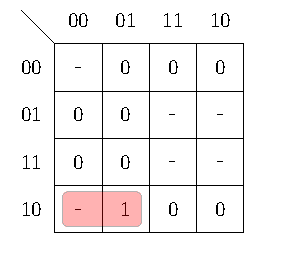
\includegraphics[scale=1.3]{S3IM1.pdf}
    \caption{Пример простейшей нейронной сети}
    \label{fig:section3:simple_nn}
\end{figure}

Искусственная нейронная сеть представляет собой совокупность соединенных и взаимодействующих
друг с другом вычислительных узлов, называемых искусственными нейронами.
Каждый нейрон получает некоторый набор сигналов, с которыми он взаимодействует,
после чего отправляет сигналы другим нейронам. В общем случае, нейрон с $n$ входами
можно описать как функцию $\mathbb{R}^{n} \rightarrow \mathbb{R}$, которая преобразует несколько
входных параметров в один выходной.
На рисуке \ref{fig:section3:neuron} изображена схема искусственного нейрона.

\begin{figure}[h!]
    \centering
    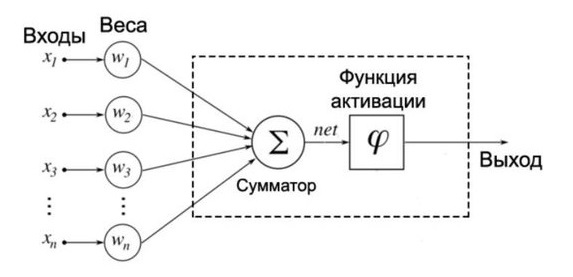
\includegraphics[scale=1.3]{S3IM2.jpg}
    \caption{Схема искусственного нейрона}
    \label{fig:section3:neuron}
\end{figure}

Как видно из рисунка, у нейрона есть $n$ входов $x_i$, у каждого  из которых
есть вес $w_i$, на который умножается сигнал, проходящий по данной связи.
После этого взвешенные сигналы $w_i \cdot x_i$ суммируются, в результате чего
получается взвешенная сумма $net$. 
Полученное значение подается в функцию активации $\varphi$, 
после чего преобразованное значение подается на выход нейрона.

Существует множество архитектур нейронных сетей, 
предназначенных для эффективного решения определенных задач.

Рассматриваемая в рамках работы задача шумоподавления относится к задачам распознавания образов.

Для решения задач распознавания образов и классификации используются следующие
архитектуры:
\begin{itemize}
    \item Сети прямого распространения.
    \item Сверточные нейронные сети.
    \item Сети адаптивного резонанса.
    \item Сети радиально-базисных функций.
\end{itemize}

Сети прямого распространения и сверточные нейронные сети используют способ
обучения с учителем, поэтому являются наиболее подходящими для решения
задачи шумоподавления, где в качестве
обучающей выборки используются определенные звуковые сигналы
с обозначенными в них источниками шума.

\subsection{Сети прямого распространения}

Сеть прямого распространения -- это нейронная сеть, сигналы в которой распостраняются
строго от входа к выходу.

На рисунке \ref{fig:section3:feed_forward} приведен пример нейронной сети
прямого распространения сигнала.

\begin{figure}[h!]
    \centering
    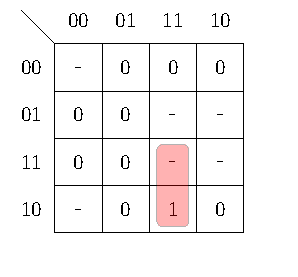
\includegraphics[scale=1]{S3IM3.pdf}
    \caption{Пример сети прямого распространения}
    \label{fig:section3:feed_forward}
\end{figure}

Как правило, под сетями прямого распространения подразумевают
полносвязные многослойные нейронные сети с прямым распространением сигнала.

Многослойная нейронная сеть -- это сеть, содержащая более одного скрытого слоя.

Полносвязная нейронная сеть -- это сеть, в которой каждый нейрон соединен со всеми
нейронами предыдущего слоя.

В дальнейшем многослойную полносвязную нейронную сеть прямого распространения
будем называть классической.

\subsection{Метод обратного распространения ошибки}

Основным методом обучения многослойных нейронных сетей является
метод обратного распространения ошибки.

Метод обратного распространения ошибки -- алгоритм обучения 
многослойных сетей прямого распространения и относится 
к методам обучения с учителем \cite{galushkin}.

В основе идеи алгоритма лежит использование выходной ошибки нейронной сети.

Под выходной ошибкой нейронной сети понимают степень отклонения выходных значений
сети от целевых значений.

Ниже представлена формула среднеквадратичной выходной ошибки нейронной сети:

\begin{equation*}
    \textstyle E = \frac{1}{2}\sum_{i = 1}^{n} (y_{i} - y_{i}^{*})^2,
\end{equation*}

\begin{explanation}
    \item[где] $n$ - число выходных нейронов;
    \item $y_{i}$ - целевое значение;
    \item $y_{i}^{*}$ - фактическое выходное значение. 
\end{explanation}

На каждой итерации обучения происходит два прохода сети: прямой и обратный.
На прямом проходе входной вектор сигналов распространяется от входов
сети к её выходам и формирует некоторый выходной вектор, соответствующий
текущему набору весов сети. 

После того, как был вычислен выходной вектор, вычисляется выходная ошибка
нейронной сети.

На обратном проходе эта выходная ошибка распространяется от выходов сети к
её входам, после чего производится коррекция весов сети.

Первым этапом является вычисление отклонения для каждого нейрона слоя:

\begin{equation}
    \textstyle \delta_{i} = \varphi^{'}(x) (y - y^{*})
    \label{eq:section3:delta_o}
\end{equation}
%
\begin{equation}
    \textstyle \delta_{i} = \varphi^{'}(x) \sum_{j = 1}^{n} (w_{i,j} \delta_{i})
    \label{eq:section3:delta_h}
\end{equation}

Так как у выходного нейрона нет исходящих связей, для расчета его отклонения
используется формула (\ref{eq:section3:delta_o}), 
в то время как для расчета отклонения скрытого нейрона 
используется формула (\ref{eq:section3:delta_h}).

На следующем этапе вычисляется градиент для связи между нейронами:

\begin{equation*}
    \textstyle grad_{i,j} = \delta_{j} y_{i},
\end{equation*}

\begin{explanation}
    \item[где] $i$ - начало связи;
    \item $j$ - конец связи.
\end{explanation}

Заключительным этапом является вычисление изменения веса связи между нейронами:

\begin{equation*}
    \textstyle \varDelta w_{i, j} = \eta grad_{i, j} + \alpha \varDelta w_{i, j}^{*},
\end{equation*}

\begin{explanation}
    \item[где] $\eta$ - скорость обучения ($0 < \eta < 1$);
    \item $\alpha$ - момент обучения ($0 < \alpha < 1$);
    \item $\varDelta w_{i, j}$ - текущее изменение веса;
    \item $\varDelta w_{i, j}^{*}$ - предыдущее изменение веса.
\end{explanation}

Описанный выше способ вычисления дельт называется градиентным
методом и заключается в вычислении градиентов весов связей
для минимизации отклонения выхода нейрона от целевого выходного значения.
Основным преимуществом данного метода является простота и наглядость
производимых вычислений.

При вычислении дельт по формулам, представленным выше, используется стохастический
метод обновления весов, суть которого заключается в обновлении веса связи
сразу после вычисления его дельты.

\subsection{Сверточные нейронные сети}

Сверточная нейронная сеть -- это специальная архитектура нейронных сетей,
нацеленная на эффективное распознавание образов. Впервые модель сверточных нейронных сетей была предложена в 1988 году 
Яном Лекуном \cite{lecun}.

Модель сверточных нейронных сетей использует в себе некоторые особенности
зрительной коры головного мозга, в которой были обнаружены
простые клетки, реагирующие на световые лучи под разными углами,
и сложные клетки, реакция которых связана с активаций определенных групп
простых клеток \cite{matsugu}.

Основными видами слоев в сверточных нейронных сетях являются
сверточые (convolutional), пулинговые (pooling) и полносвязные (dense) слои.
На рисунке \ref{fig:section3:simple_cnn} изображена сверточная нейронная сеть,
состоящая из 4 сверточных, 4 пулинговых и 1 полносвязного слоя.

\begin{figure}[h!]
    \centering
    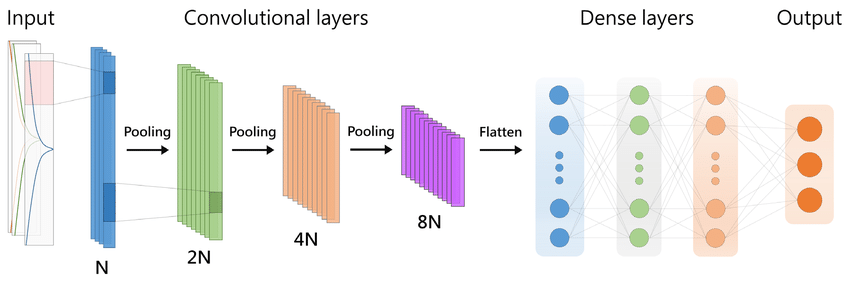
\includegraphics[scale=0.55]{S3IM4.png}
    \caption{Пример сверточной нейронной сети}
    \label{fig:section3:simple_cnn}
\end{figure}

Свертка -- бинарная операция над матрицами, 
суть которой заключается в том, 
что каждый фрагмент первой матрицы поэлементно умножается на вторую матрицу, 
результаты суммируются и записываются 
в соответствующую позицию итоговой матрицы.

Формально операцию свертки над матрицами A и B можно представить следующими
формулами:

\begin{equation*}
    C(n_x - m_x + 1; n_y - m_y + 1) = A(n_x; n_y) * B(m_x, m_y),
\end{equation*}
%
\begin{equation*}
    \textstyle C_{i,j} = \sum_{u = 0}^{m_x - 1} \sum_{v = 0}^{m_y - 1} A_{i + u, j + v} B_{u, v}
\end{equation*} 

На рисунке \ref{fig:section3:convolution} изображен пример
выполнения операции свертки над матрицами 
$\textstyle 7 \times 7$ и $3 \times 3$.

\begin{figure}[h!]
    \centering
    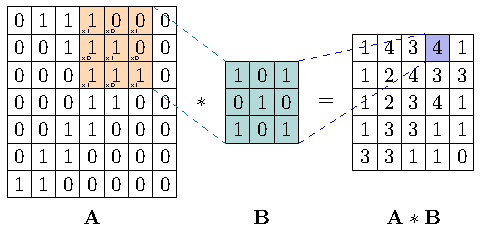
\includegraphics[scale=1.25]{S3IM5.pdf}
    \caption{Пример выполнения операции свертки}
    \label{fig:section3:convolution}
\end{figure}

Операция свертки является основным преимуществом сверточных нейронных сетей.
В отличие от перцептронов, где каждый нейрон связан со всеми нейронами предыдущего
слоя определенными весовыми коэффициентами, в сверточной нейронной сети
для различных нейронов выходного слоя используется одна и та же матрица весов,
называемая \emph{ядром свертки}. Интерпретацией такого подхода является
графическое кодирование какого-либо признака, например, наличие определенного набора
пикселей на участке изображения. При этом ядра свертки не закладываются
в архитектуру заранее, а формируются при обучении 
\emph{методом обратного распространения ошибки}.  

Операция пулинга -- операция,
выполняющая уменьшение размерности сформированных под действием операции
свертки карт признаков. Исходная матрица делится на блоки размером 
$\textstyle w \times h$, 
для каждого из которых вычисляется некоторая функция.

На рисунке \ref{fig:section3:pooling} изображен пример выполнения 
операции пулинга $\textstyle 2 \times 2$ с функцией максимума.

\begin{figure}[h!]
    \centering
    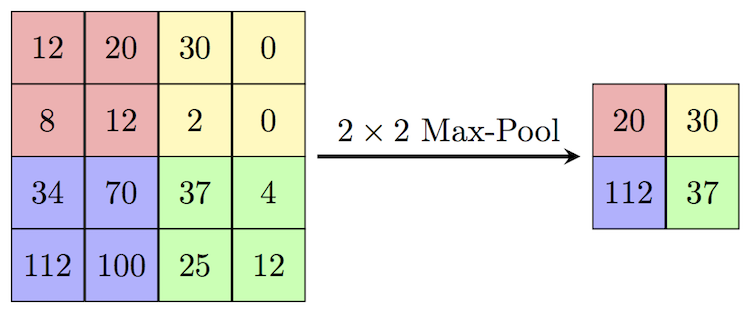
\includegraphics[scale=1.8]{S3IM6.png}
    \caption{Пример выполнения операции пулинга}
    \label{fig:section3:pooling}
\end{figure}

После нескольких прохождений слоев свертки и пулинга исходная матрица
высокого разрешения преобразуется к более абстрактным картам признаков,
причем, как правило, на каждом следующем слое 
увеличивается число карт и уменьшаются их размеры.
В результате остается большой набор каналов, хранящих небольшое 
число данных, которые интерпретируются как признаки, выявленные
из исходного изображения.
Данные на каналах объединяются и подаются на вход 
обычной полносвязной нейронной сети, 
по которым она выполняет задачу 
распознавания или классификации исходных данных.

\subsection{Преимущества сверточных нейронных сетей}

Сверточные нейронные сети имеют ряд преимуществ,
среди которых можно выделить следующие:

\begin{itemize}
    \item Сверточные нейронные сети более эффективно распознают
    и классифицируют изображения.

    \item По сравнению с полносвязными нейронными сетями
    сверточные нейронные сети имеют гораздо меньшее количество
    настраиваемых весов, что связано с наличием сверточных слоев.
    Такой подход подталкивает сеть к обобщению демонстрируемой
    информации и поиску закономерностей, 
    а не к попиксельному запоминанию обрабатываемых изображений.

    \item Удобное распараллеливание вычислений дает возможность
    повысить скорость выполнения алгоритмов работы и обучения сети.

    \item Устойчивость к линейным преобразованиям
    распознаваемого изображения (к масштабированию, повороту, сдвигу).
\end{itemize}